\documentclass{vgtc}                          % final (conference style)
\ifpdf
  \pdfoutput=1\relax
  \pdfcompresslevel=9
  \pdfoptionpdfminorversion=7
  \ExecuteOptions{pdftex}
  \usepackage{graphicx}
  \DeclareGraphicsExtensions{.pdf,.png,.jpg,.jpeg}
\else
  \ExecuteOptions{dvips}
  \usepackage{graphicx}
  \DeclareGraphicsExtensions{.eps}
\fi
\graphicspath{{figures/}{pictures/}{images/}{./}}
\PassOptionsToPackage{warn}{textcomp}
\usepackage{microtype}
\usepackage{textcomp}
\usepackage{mathptmx}
\usepackage{times}
\usepackage{cite}
\usepackage{tabu}
\usepackage{booktabs}
\usepackage{amsmath}
\usepackage[nolist]{acronym}
\usepackage{listings}
\usepackage[table,xcdraw]{xcolor}
\usepackage{booktabs}
\usepackage{array}
\usepackage{multirow}
\usepackage{steinmetz}
\usepackage[final]{pdfpages}
\usepackage[abbreviations]{glossaries-extra}
\usepackage{booktabs}
\usepackage{xspace}
\usepackage{color}
\usepackage{xcolor}
\usepackage{savesym}
\usepackage{setspace}
\usepackage{tikz}
\usepackage{colortbl}
\usepackage{enumitem}
\input{listings}

\savesymbol{spacing}
\definecolor{Orange}{rgb}{1.0, 0.5, 0.0}
\definecolor{DarkGreen}{rgb}{0, 0.5, 0.0}
\definecolor{Purple}{rgb}{0.7, 0.0, 0.7}
\definecolor{Blue}{rgb}{0.2, 0.2, 0.8}
\definecolor{Red}{rgb}{1.0, 0.0, 0.0}
\definecolor{Brown}{rgb}{0.7, 0.4, 0.1}
\definecolor{Blue}{rgb}{0, 0, 1.}
\definecolor{Green}{rgb}{0., 0.6, 0.}
\definecolor{Custom}{rgb}{0.3, 0.1, 0.2}
\definecolor{Yellow}{rgb}{0.9, 0.7, 0.0}
\definecolor{Purple}{rgb}{0.9, 0.1, 0.8}

\renewcommand*\ttdefault{txtt}
\newcommand{\etal}{~et al.\@\xspace}
\newcommand{\etc}{etc.\@\xspace}
\newcommand{\eg}{e.g.\@\xspace}
\newcommand{\Eg}{E.g.\@\xspace}
\newcommand{\ie}{i.e.\@\xspace}
\newcommand{\Ie}{I.e.\@\xspace}
\newcommand{\Fig}{Fig.\@\xspace}
\newcommand{\fig}{Fig.\@\xspace}
\newcommand{\projectname}{\textit{HoloBeam}\@\xspace}
\newcommand{\codebase}{\textcolor{blue}{\href{https://github.com/complight/multiholo}{GitHub:complight/multiholo}}\@\xspace}
\newcommand{\NewEmptyPage}{\newpage\null\thispagestyle{empty}\newpage}
\newcommand{\high}[1]{{\cellcolor{green!25} #1}}
\newcommand{\medium}[1]{\cellcolor{yellow!25} #1}
\newcommand{\low}[1]{\cellcolor{red!25} #1}

\newabbreviation{cpd}{cpd}{Cycles Per Degree}
\newabbreviation{SLM}{SLM}{Spatial Light Modulator}
\newabbreviation{HVS}{HVS}{Human Visual System}
\newabbreviation{DMD}{DMD}{Digital Micromirror Device}
\newabbreviation{AR}{AR}{Augmented Reality}
\newabbreviation{VR}{VR}{Virtual Reality}
\newabbreviation{CGH}{CGH}{Computer-Generated Holography}
\newabbreviation{FoV}{FoV}{Field Of View}
\newabbreviation{HOE}{HOE}{Holographic Optical Element}
\newabbreviation{3D}{3D}{Three-Dimensional}
\newabbreviation{CNN}{CNN}{Convolutional Neural Network}
\newabbreviation{MTF}{MTF}{Modulation Transfer Function}

\global\long\def\MTF{\gls{MTF}\xspace}
\global\long\def\CNN{\gls{CNN}\xspace}
\global\long\def\HVS{\gls{HVS}\xspace}
\global\long\def\3D{\gls{3D}\xspace}
\global\long\def\cpd{\gls{cpd}\xspace}
\global\long\def\SLM{\gls{SLM}\xspace}
\global\long\def\AR{\gls{AR}\xspace}
\global\long\def\VR{\gls{VR}\xspace}
\global\long\def\CGH{\gls{CGH}\xspace}
\global\long\def\HOE{\gls{HOE}\xspace}
\global\long\def\FoV{\gls{FoV}\xspace}
\global\long\def\DMD{\gls{DMD}\xspace}
\global\long\def\ARs{\gls{AR}s\xspace}
\global\long\def\VRs{\gls{VR}s\xspace}
\global\long\def\CGHs{\gls{CGH}s\xspace}
\global\long\def\HOEs{\gls{HOE}s\xspace}
\global\long\def\FoVs{\gls{FoV}s\xspace}
\global\long\def\SLMs{\gls{SLM}s\xspace}
\global\long\def\DMDs{\gls{DMD}s\xspace}

\newcommand{\refSec}[1]{Sec.~\ref{sec:#1}}
\newcommand{\refFig}[1]{Fig.~\ref{fig:#1}}
\newcommand{\refEq}[1]{Eq.~\ref{eq:#1}}
\newcommand{\refTbl}[1]{Tbl.~\ref{tbl:#1}}
\newcommand{\refObj}[1]{Objective~\ref{obj:#1}}

\onlineid{1231}
\vgtccategory{Research}
\vgtcinsertpkg
\ieeedoi{xx.xxxx/TVCG.201x.xxxxxxx}
\title{HoloBeam: Paper-Thin Near-Eye Displays}
\author{Kaan Akşit\thanks{e-mail: k.aksit@ucl.ac.uk}\\ %
        \scriptsize University College London %
\and Yuta Itoh\thanks{e-mail: yuta.itoh@iii.u-tokyo.ac.jp}\\ %
     \scriptsize The University of Tokyo %
}
\teaser{
\centering
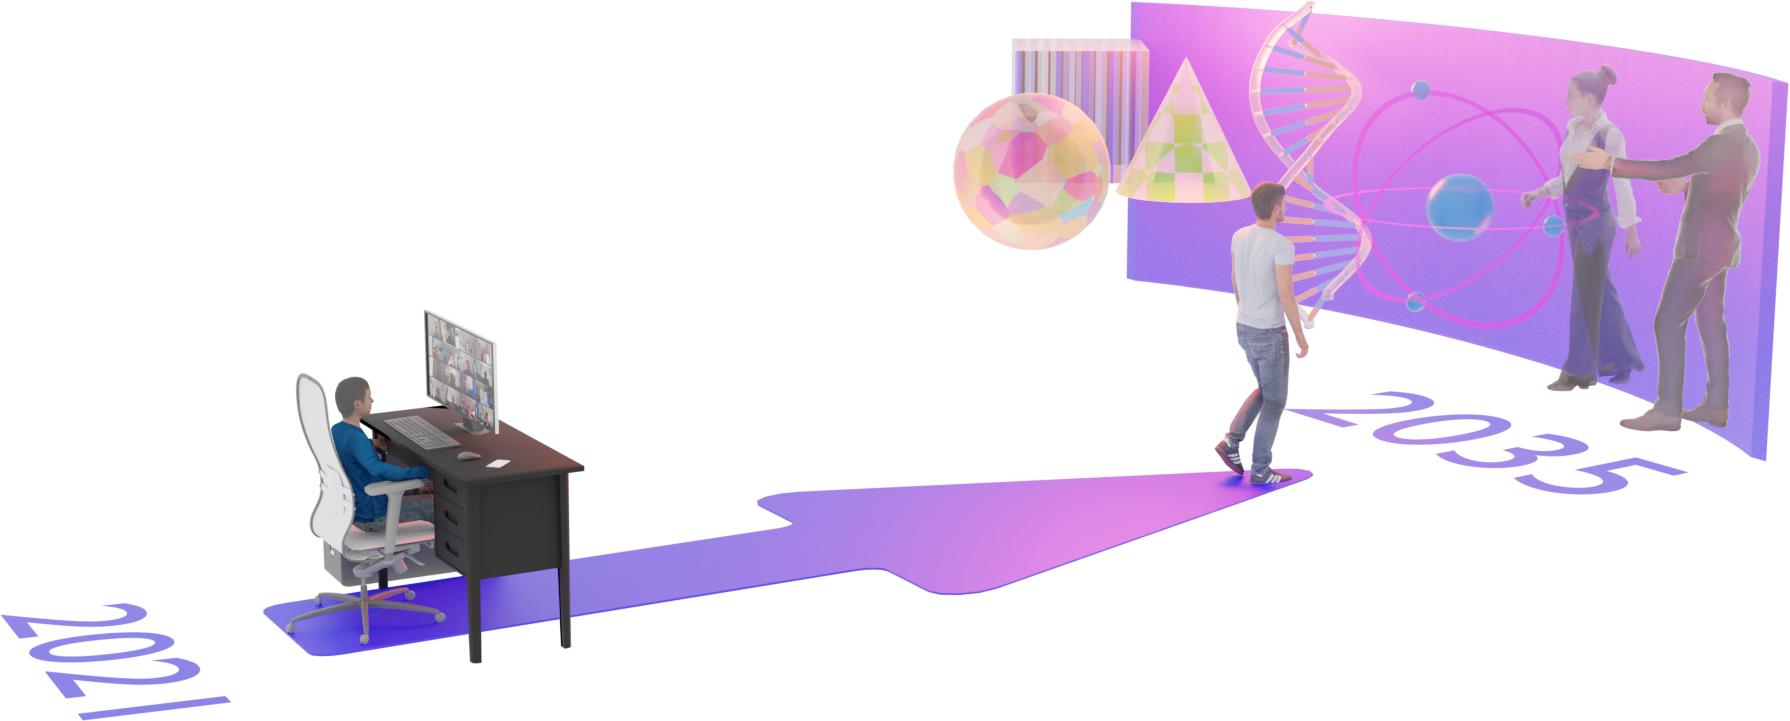
\includegraphics[width=\linewidth]{figures/teaser.png}
\caption{
\projectname slim Virtual Reality headsets and Augmented Reality glasses with wide field of view and high resolutions.
(a) Layout. A light beam from a light source gets modulated by a Spatial Light Modulator (SLM).
Modulated beam reconstructs multiplane images in the vicinity of SLM (a few millimeters away).
With the help of multiple lenses forming a projection system, conjugate images are formed at considerable throw distances (e.g., a few tens of cm to a meter or two).
These conjugate images are relayed to a user's retina with the help of a slim and lightweight eyepiece.
Thus, users can perceive high-resolution \3D virtual images overlayed on their real-world scene.
(b) Wearable Eyepiece.
\projectname glasses is made of wearable eyepieces that could come in the form of a submillimeter-thick holographic optical elements or conventional lenses with a reasonable thickness.
(c) A view from eyebox.
Provided photograph demonstrates the high image quality and wide field of view of a phase-only modulating \projectname prototype when viewed through eyepieces that use conventional lenses.
Source image is from Flicker user gags9999.
}
\label{fig:teaser}
}

\abstract{
An emerging alternative to conventional Augmented Reality (AR) glasses designs, Beaming displays promise slim AR glasses free from challenging design trade-offs, including battery-related limits or computational budget-related issues.
These beaming displays remove active components such as batteries and electronics from AR glasses and move them to a projector that projects images to a user from a distance (1-2 meters), where users wear only passive optical eyepieces.
However, earlier implementations of these displays delivered poor resolutions (7 cycles per degree) without any optical focus cues and were introduced with a bulky form-factor eyepiece ($\sim50~mm$ thick).
This paper introduces a new milestone for beaming displays, which we call \projectname.
In this new design, a custom holographic projector populates a micro-volume located at some distance (1-2 meters) with multiple planes of images.
Users view magnified copies of these images from this small volume with the help of an eyepiece that is either a Holographic Optical Element (HOE) or a set of lenses.
Our \projectname prototypes demonstrate the thinnest AR glasses to date with submillimeter thickness (\eg, HOE film is only $120~\mu m$ thick).
In addition, \projectname prototypes demonstrate near retinal resolutions ($24$ cycles per degree) with a $70$ degrees-wide field of view.
}
%% ACM Computing Classification System (CCS). 
%% See <http://www.acm.org/about/class> for details.
%% We recommend the 2012 system <http://www.acm.org/about/class/class/2012>
%% For the 2012 system use the ``\CCScatTwelve'' which command takes four arguments.
%% The 1998 system <http://www.acm.org/about/class/class/2012> is still possible
%% For the 1998 system use the ``\CCScat'' which command takes four arguments.
%% In both cases the last two arguments (1998) or last three (2012) can be empty.
\CCScatlist{
  \CCScatTwelve{Hardware}{Emerging Technologies}{Emerging optical and photonic technology}{};
  \CCScatTwelve{Hardware}{Communication hardware, interfaces and storage}{Display and imagers}{}
}
%\CCScatlist{
  %\CCScat{H.5.2}{User Interfaces}{User Interfaces}{Graphical user interfaces (GUI)}{};
  %\CCScat{H.5.m}{Information Interfaces and Presentation}{Miscellaneous}{}{}
%}
\begin{document}
\firstsection{Introduction}
\label{sec:introduction}

\maketitle
Emerging as the future's interface~\cite{orlosky2021telelife}, \VR and \AR glasses are expected to redefine how we interact with real and virtual environments by overlaying rendered images within our visual \FoV.
To achieve this vision, recent years have seen a strong push from the scientific community to build \AR \cite{maimone2017holographic, maimone2014pinlight} and \VR \cite{ratcliff2020thinvr,kim2022holographicglasses} glasses that are thin and lightweight.
Video see-through \AR~\cite{ebner2022video} and \VR headsets block the real-world view, whereas optical see-through \AR has no such luxury to do so.
Expectation from both \AR glasses and \VR headsets is that they should support high resolutions, wide \FoV, and optical focus cues \cite{aghasi2021optimal}.
To date, \VR headsets and AR glasses in the literature have struggled to balance these requirements, often yielding to issues related to one or more requirements (e.g., slim but low \FoV, bulky but with optical focus cues).


An emerging design alternative to conventional designs for AR glasses, Beaming Displays~\cite{itoh2021beaming}, argues that designs should separate active and passive parts in AR glasses into two discrete components.
Specifically, these Beaming Displays project images from a distance (1-2 m) to a user wearing a passive lightweight optical eyepiece.
Thanks to removing active components from AR glasses, Beaming Displays fundamentally avoid heating, computation, and power budget-related issues.
At the core, Beaming Displays aim to balance design requirements such as form-factor, resolution, \FoV, and optical focus cues.
However, the previous implementation of Beaming Displays~\cite{itoh2021beaming} provided a limited resolution with 7 \cpd and 50~mm thick bulky AR glasses.
Thus, the promises of Beaming Displays have yet to be fully realized.

\begin{table*}[ht!]
  \caption{
Comparison between \AR and \VR near-eye displays. Here, focus refers to the method used to support the optical focus cues. Optical see-through refers to the level of see-through in the real world. Wide eye-box refers to supporting varying gazes of users (above 10 mm). Moderate monocular fields of view are 20-50 degrees. Moderate resolution matches 10-20 cycles per degree. Although our work offers no mobility, it distinguishes itself as the slim and lightweight AR near-eye display, free from heating issues or limited power and computing resources.
         }
  \label{tbl:comparison}
  \begin{tabular}{m{2.9cm} m{1.2cm} m{1.0cm} m{0.6cm} m{1.0cm} m{1.0cm} m{1.43cm} m{0.82cm} m{1.3cm} m{1.1cm} m{0.8cm}}
    \toprule
	  & Focus & See-through & Eyebox & Field of View & Resolution & Form factor & Weight & Power and Compute & Heat & Mobility\\
    \midrule


          This work & 
          \high{CGH} & 
          \high{Clear} & 
          \low{Small} &
          \high{Wide} & 
          \high{High} & 
          \high{Paper-Thin} & 
          \high{Light} & 
          \high{Expandable} & 
          \high{No issue} &
          \low{Fixed}
          \\ \hline


	  Beaming Displays \cite{itoh2021beaming} & 
	  \low{Fixed} & 
	  \medium{Moderate} & 
          \high{Wide} &
	  \medium{Moderate} & 
	  \low{Low} & 
	  \low{Bulky} & 
	  \low{Regular} & 
	  \high{Expandable} & 
	  \high{No issue} &
	  \medium{Limited}
	  \\ \hline


	  Holographic VR \cite{kim2022holographicglasses}& 
	  \high{CGH} & 
	  \low{Blocks} & 
	  \low{Small} &
	  \high{Wide} & 
	  \high{High} & 
	  \medium{Thin} & 
	  \low{Regular} & 
	  \low{Limited} & 
	  \low{Issue} &
	  \high{Mobile}
	  \\ \hline


	  Video MR \cite{ebner2022video}& 
	  \high{Multiplane} & 
	  \medium{Video} & 
	  \high{Wide} &
	  \medium{Moderate} & 
	  \medium{Moderate} & 
	  \low{Bulky} & 
	  \low{Regular} & 
	  \low{Limited} & 
	  \low{Issue} &
	  \high{Mobile}
	  \\ \hline


	  Wide Étendue \cite{kuo2020high} & 
	  \high{CGH} & 
	  \medium{Moderate} & 
	  \high{Wide} &
	  \high{Wide} & 
          \low{Low} & 
	  \low{Bulky} & 
	  \low{Regular} & 
	  \low{Limited} & 
	  \low{Issue} &
	  \high{Mobile}
	  \\ \hline


	  Foveated AR \cite{kim2019foveated} & 
	  \high{Varifocal} & 
	  \medium{Moderate} & 
	  \low{Small} &
	  \high{Wide} & 
	  \high{High} & 
	  \low{Bulky} & 
	  \low{Regular} & 
	  \low{Limited} & 
	  \low{Issue} &
	  \high{Mobile}
	  \\ \hline


          Scanning Eyebox \cite{jang2018holographic} & 
	  \high{CGH} & 
	  \high{Clear} & 
	  \high{Wide} & 
	  \medium{Moderate} &
	  \medium{Moderate} & 
	  \low{Bulky} & 
	  \low{Regular} & 
	  \low{Limited} & 
	  \low{Issue} &
	  \high{Mobile}
	  \\ \hline



	  Varifocal AR \cite{akcsit2017near}& 
	  \high{Varifocal} & 
	  \medium{Moderate} & 
	  \high{Wide} &
	  \high{Wide} & 
	  \medium{Moderate} & 
	  \low{Bulky} & 
	  \low{Regular} & 
	  \low{Limited} & 
	  \low{Issue} &
	  \high{Mobile}
	  \\ \hline


	  Holographic AR \cite{maimone2017holographic} & 
	  \high{CGH} & 
	  \high{Clear} & 
	  \low{Small} &
	  \high{Wide} & 
	  \high{High} & 
	  \medium{Thin} & 
	  \low{Regular} & 
	  \low{Limited} & 
	  \low{Issue} &
	  \high{Mobile}
	  \\ \hline


          Lightfield VR \cite{huang2015light} & 
	  \high{Lightfield} & 
          \low{Blocks} & 
          \high{Wide} &
	  \medium{Moderate} & 
	  \low{Low} & 
	  \low{Bulky} & 
	  \low{Regular} & 
	  \low{Limited} & 
	  \low{Issue} &
	  \high{Mobile}
	  \\ \hline


          Pinlight Displays \cite{maimone2014pinlight} & 
	  \high{Lightfield} & 
          \medium{Moderate} & 
          \low{Small} &
	  \medium{Moderate} & 
	  \low{Low} & 
	  \medium{Thin} & 
	  \low{Regular} & 
	  \low{Limited} & 
	  \low{Issue} &
	  \high{Mobile}
	  \\ \hline


          Microlens VR \cite{lanman2013near} & 
	  \high{Lightfield} & 
          \low{Blocks} & 
          \low{Small} &
	  \low{Narrow} & 
	  \low{Low} & 
	  \medium{Thin} & 
	  \low{Regular} & 
	  \low{Limited} & 
	  \low{Issue} &
	  \high{Mobile}
	  \\


    \bottomrule
  \end{tabular}
\vspace{-3mm}
\end{table*}


Our code  is available at \codebase.
Additional media, results and materials are distributed separately as a supplementary documents.



\bibliographystyle{abbrv-doi}
\bibliography{references}

\end{document}

